\chapter{Hardware Acceleration of Convolutional Neural Networks}
\label{ch3_cnn}
Deep Learning is an avant-garde approach to imparting knowledge to the machines to achieve the ultimate goal of artificial intelligence without explicit coding, and bridge the current gap between technology integration and expertise. It is of interest in several domains\cite{wiki_ml}, such as:
\begin{itemize}
\item Self-driving cars, Automated flight control, Handwriting and Voice recognition software, which are real-time and cannot be programmed by hand or require intense effort doing so manually.
\item Database Mining.
\item Applications with Product Recommendations in e-commerce websites such as Amazon and Netflix, which are essentially self-customizing.
\item Understanding of the human genome.
\item Anti-Spam filters and Intelligent Search bars in browsers.
\end{itemize} 
Claims have been made that off-the-shelf accelerators in the embedded platforms offer an edge over CPU-based systems in deep learning computations\cite{hegde2016caffepresso}. We seek to validate the efficiency of deep-learning methods on heterogeneous architectures with a simple Lenet-5 Model of MNIST Dataset classifier. 
\section{Deep Learning using Convolutional Neural Networks}
\label{3_1}
The Figure \ref{fig:ML_Classification} shows the most common types of learning algorithms. The choice of the algorithm depends on the problem we intend to solve.
\begin{figure}[h!]
  \centering
  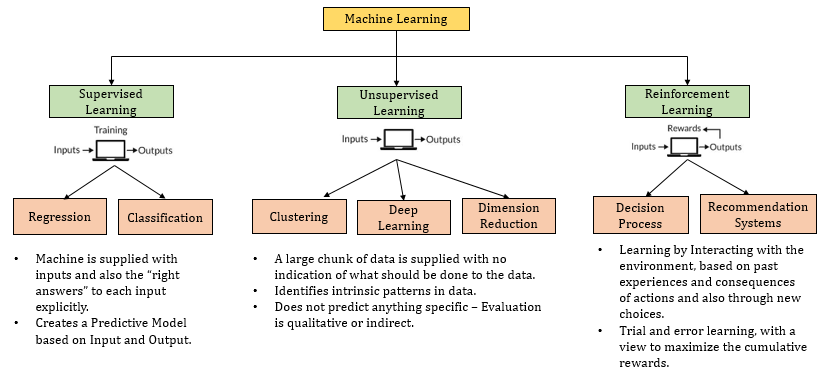
\includegraphics[width=\linewidth]{figures/ML_Classification.PNG}
  \caption{Types of Machine Learning Algorithms
  \cite{upx_ml}}
  \label{fig:ML_Classification}
\end{figure}
\newline Various experiments have substantiated the claim that Convolutional Neural Networks (also called ConvNets or CNNs) outperform other gradient-based learning techniques in handling variable input dimensions in the 2-dimensional space \cite{lecun1998gradient}.
Multilayer ConvNets with back-propagation can be exploited to build a strong decision layer capable of classifying data of high dimensionality, with minimal processing. \newline \newline
Any character recognition system is comprised of the following two parts:\newline
1.	\textbf{Feature Extractor }– \newline
It transforms the input into low-dimensional feature vectors which comprise of only the relevant information of interest from the huge input data \cite{wiki_fe}. The chosen features are essentially invariant to the transformations and distortions that are applied to the input. 
\newline
Feature extraction attempts to reduce the complexity that stems from high input dimensionality, by downsizing the data while still accomplishing reasonable accuracy in the description of data \cite{wiki_fe}. Feature extractors are application-specific.\newline \newline
2.	\textbf{Classifier} – \newline
It is a trainable general-purpose entity which analyzes the data and categorizes the feature vectors appropriately into classes. The accuracy of a classifier is predominantly decided by the features selected in the feature extraction process. \newline
The efficiency of a classifier is determined not just by the correctness in categorizing a given set of test input samples but also the error rate. 
\begin{figure}[h!]
  \centering
  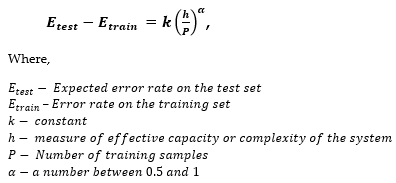
\includegraphics[width=0.7\linewidth]{figures/classifier_efficiency_formula.PNG}
  \caption{Formula to determine Classifier Efficiency
  \cite{lecun1998gradient}}
  \label{fig:classifier_efficiency_formula}
\end{figure}
\newline Studies have revealed the relationship between expected error rate on test set and error rate on training set as shown in Figure \ref{fig:classifier_efficiency_formula}. The difference between these two error values decreases as the number of training samples increases. Also, if the complexity of the system “h” increases, training error decreases. Hence, we infer that the system becomes more robust with more training. 
\newline \newline
The traditional machine learning approach involves handcrafting features of interest, which can take painstaking amount of time and effort, coupled with domain expertise. Feature engineering in Deep nets is automatic and more accurate in comparison to conventional methods \cite{dlintro_am}.
\begin{figure}[h!]
  \centering
  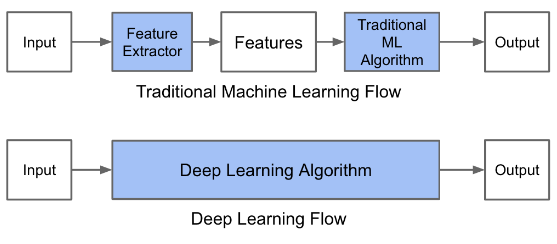
\includegraphics[width=0.7\linewidth]{figures/dlvsml.png}
  \caption{Learning differences - Traditional vs. Deep Learning
  \cite{dlintro_am}}
  \label{fig:deep_learning_flow}
\end{figure}
\newline
Owing to high computational complexity, CNN usage is restricted, especially in portable devices \cite{gysel2016hardware}. 

\subsection{MNIST Digit Recognition using Lenet-5 ConvNet}
\label{3_1_1}
The Lenet-5 Architecture for handwritten digit recognition was first conceived by LeCun et al. in 1998. The MNIST(Modified National Institute of Standards and Technology) database consisting of 60000 training samples and 10000 test inputs available for download in \cite{mnist_database} was used for the experiments discussed in the paper \cite{lecun1998gradient}. This paper proved the general consensus \ref{fig:deep_learning_flow}  that ConvNets eliminate the need for hand-made feature extractors and are the most efficient. Today, Artificial Intelligence is a buzzword and almost all AI related applications are leveraging ConvNets to achieve the best performance with low runtime complexities. 
\begin{figure}[h!]
  \centering
  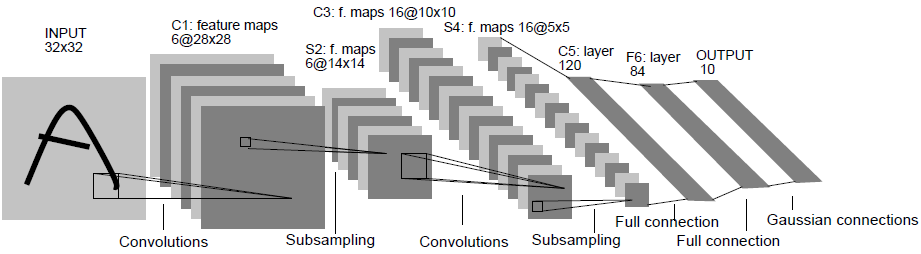
\includegraphics[width=\linewidth]{figures/Lenet-5-org.PNG}
  \caption{Original Lenet-5 ConvNet Architecture; Each plane represents a feature map in which weights are shared.
  \cite{lecun1998gradient}}
  \label{fig:Lenet-5-org}
\end{figure}
Figure \ref{fig:Lenet-5-org} shows the original Lenet-5 architecture described in \cite{lecun1998gradient}. 
It is important to understand the purpose of various layers of the Lenet-5 ConvNet architecture to study their runtime in the application. The following subsections shall describe the layers in detail.
\subsubsection{Convolution Layer \cite{cnn_ak}}  
\begin{figure}[h!]
  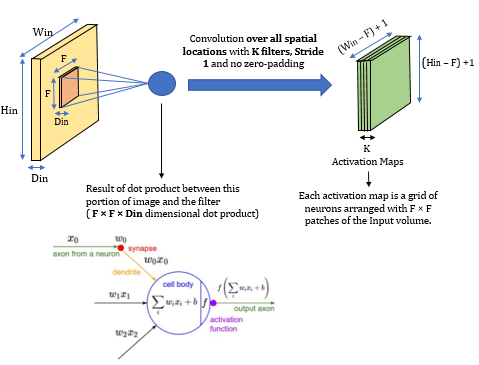
\includegraphics[width=\linewidth]{figures/ConvLayer.PNG}
  \caption{Convolution Layer
  \cite{cnn_ytak}}
  \label{fig:ConvLayer}
\end{figure}
Convolution Layer is the core of a ConvNet. Consider an input volume of height $H_i$, width $W_i$ and depth $D_i$. The depth indicates the color channels, i.e. the third dimension of input volume which can be activated. A filter of dimension F × F is slid over the input image spatially to evaluate dot products between the input image volume and the filter, thus generating 2-dimensional activation maps. The filter spans through the depth of the input image. 
\newline \newline Activation map is a visualization of which portions of the input volume are responding to the filter. For example, if the filter is intended to filter out vertical lines, activation map is representative of filter activations on the image. i.e. it contains all portions of the image which are likely to have vertical lines.  Usually, several filters, also called kernels are convolved with the input image, resulting in several activation maps stacked in the depth dimension. In a ConvNet, there are several convolution layers and intuitively, they build up an entire feature hierarchy. 
\newline
Each stage builds up very specific features which filters in the subsequent stages will be excited about. i.e. piece by piece, we create 3-D volumes of higher levels of abstraction than the previous stage\cite{zeiler2014visualizing}.\newline \newline
\begin{figure}[h!]
  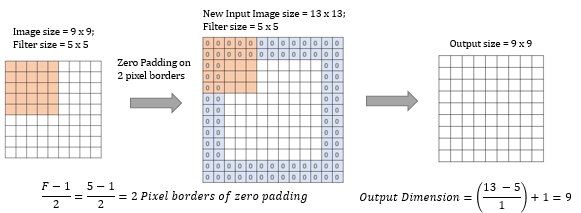
\includegraphics[width=\linewidth]{figures/zero_padding_conv.PNG}
  \caption{Preserving Input dimensions using Zero Padding
  \cite{cnn_ytak}}
  \label{fig:zero_padding_conv}
\end{figure}\underline{\textbf{\emph{\large Generalization of Concepts:}}}\newline
\textbf{Required Hyperparameters:}
	\begin{adjustwidth}{2cm}{}
       Number of filters, K \newline
       Spatial Extent of the filter, F \newline
       Stride, S \newline
       Quantum of Zero padding, P (Figure \ref{fig:zero_padding_conv})
	\end{adjustwidth}
\textbf{Input Dimensions:} $W_1$×$H_1$×$D_1$ \newline
\textbf{Output Dimensions:} $W_2$×$H_2$×$D_2$, 
	\begin{adjustwidth}{2cm}{}
      Where \newline 
	  $D_2$ = K \newline
	  $W_2$ = (($W_1$ – F +2P)/S) + 1 \newline
	  $H_2$ = (($H_1$ – F +2P)/S) + 1 \newline
    \end{adjustwidth}
Each filter has an associated bias. The value 1 is added in the above formulae to account for that bias. Stride is the distance by which the filter is slid around the input volume.\newline
Hence, total number of parameters introduced in the neural network is given by (F . F. $D_1$) × K weights and K biases. For computational convenience, K is usually set as powers of 2. Some libraries branch into special routines when encountering powers of 2, and these routines are highly optimized and efficient for computations in a vectorized form \cite{cnn_ytak}. \newline \newline
The output of a filter covering a particular region of the input x can be interpreted to be a neuron fixed in space, which computes $w^T$x + b. The connections of the neuron are localized and this connectivity expands up to the receptive field of the neuron, given by the filter size F × F. An activation map can be perceived as a grid of neurons with shared weights and representing the dot products of each F × F patch of the input volume. As there can be multiple filters in a single convolution layer, the resultant output is a 3-D volume of neurons, as illustrated in Figure \ref{fig:ConvLayer_1}. This 3-D volume has shared parameters spatially (H×W – within the same depth slice) but across depth, the parameters are different. The neurons illustrated in the Figure \ref{fig:ConvLayer_1} are all acting on the same input patch but with different weights. 
\begin{figure}[h!]
  \centering
  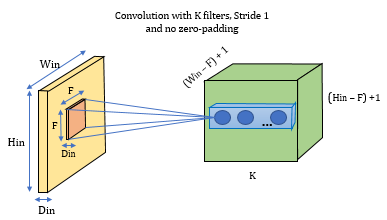
\includegraphics[width=0.7\linewidth]{figures/ConvLayer_1.PNG}
  \caption{3-dimensional volume of Neurons
  \cite{cnn_ytak}}
  \label{fig:ConvLayer_1}
\end{figure}
\subsubsection{MaxPool Layer}
\begin{figure}[h!]
\centering
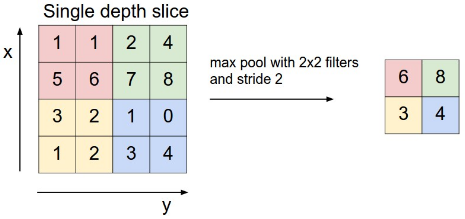
\includegraphics[width=0.7\linewidth]{figures/maxpool.PNG}
\caption{Max Pooling
\cite{cnn_ak}}
\label{fig:maxpool}
\end{figure}
Down-sampling layer which operates independently on all activation maps.
\textbf{Required Hyperparameters:}
  \begin{adjustwidth}{2cm}{}
  Spatial Extent of the filter, F \newline
  Stride, S 
  \end{adjustwidth}
\textbf{Input Dimensions:} $W_1$×$H_1$×$D_1$ \newline
\textbf{Output Dimensions:} $W_2$×$H_2$×$D_2$ 
  \begin{adjustwidth}{2cm}{}
  Where \newline
  $W_2$ = (($W_1$-F)/S)+1 \newline
  $H_2$ = (($H_1$-F)/S)+1 \newline
  $D_2$ = $D_1$
  \end{adjustwidth}
Example of Maxpool operation with filter size 2 × 2 and Stride 2 is illustrated in Figure \ref{fig:maxpool}.
\subsubsection{Inner Product Layer}
\begin{figure}[h!]
  \centering
  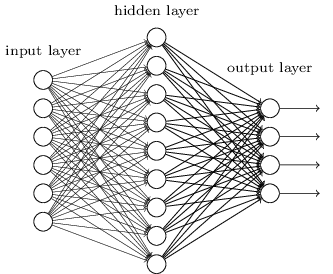
\includegraphics[width=0.5\linewidth]{figures/FCLayer.png}
  \caption{Inner Product Layer
  \cite{cnn_ak}}
  \label{fig:FCLayer}
\end{figure}
It is also called the fully connected layer as the neurons of this layer are pairwise fully connected with the neurons of the previous (input) layer. The neurons within the same layer do not share connections.
\subsubsection{ReLU Layer}
\begin{figure}[h!]
  \centering
  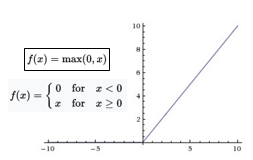
\includegraphics[width=0.5\linewidth]{figures/relu.PNG}
  \caption{ReLU Function in Neural Networks
  \cite{wiki_relu}}
  \label{fig:relu}
\end{figure}
Rectified Linear Unit \cite{nair2010rectified} is a non-linear activation function described by Figure \ref{fig:relu}, commonly used in neural networks for the purpose of thresholding after convolution. ReLU is faster compared to other activation functions such as sigmoid and tanh units as it does not involve any normalization or exponential calculation, unlike its counterparts. 
\subsubsection{Softmax Layer}
\begin{figure}[h!]
  \centering
  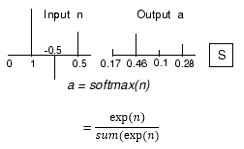
\includegraphics[width=0.3\linewidth]{figures/softmax.PNG}
  \caption{Softmax Function
  \cite{mathworks_softmax}}
  \label{fig:softmax}
\end{figure}
MNIST Digit Classifier has ten class labels for the ten digits 0 to 9, which are mutually exclusive. An ideal classifier should assign a probability of 1 to one of the ten possible nodes at the output and assign 0 probability to others. Due to difficulty in realizing this, we use Softmax function usually in the last layer of the ConvNet, which increases the probability of the maximum value from the previous stage in such a way that sum of the output probabilities of the 10 classes is 1 \cite{softmax_cmc}.
\subsubsection{Modified Hyperparameters for MNIST Dataset}
\begin{figure}[h!]
  \centering
  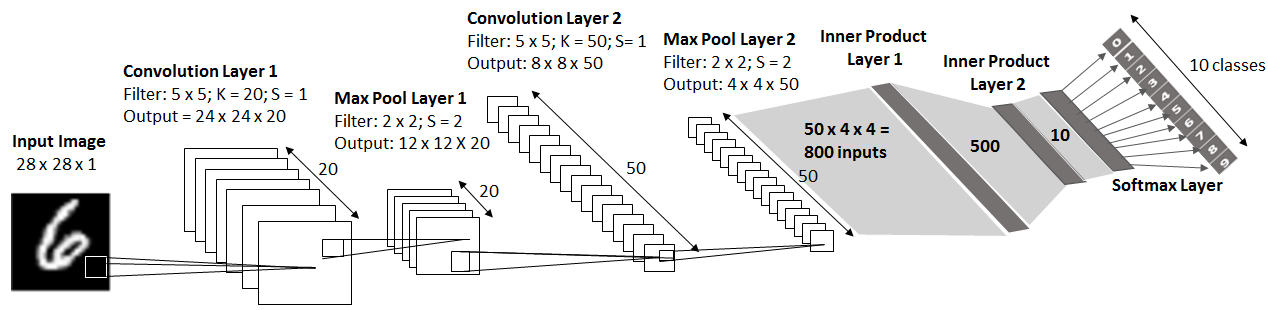
\includegraphics[width=\linewidth]{figures/Lenet-5-papaa.PNG}
  \caption{Lenet-5 CNN Architecture for MNIST Dataset with modified hyperparameters
  \cite{papaa-opencl}}
  \label{fig:Lenet-5-MNIST}
\end{figure}
Different versions of MNIST Datasets have been introduced over the years. The first version had images centred within the 28×28 region and it was extended to 32×32 images by adding extra background pixels \cite{lecun1998gradient}. In the later versions of the database, images were normalized in size to fit a 20×20 field, forming the centre of mass of the resultant 28×28 image. The Architecture illustrated in the Figure \ref{fig:Lenet-5-org} uses 32×32 images while the benchmark code \cite{papaa-opencl} that will be used for our experiments uses 28x28 images. Table \ref{table:hyperparams} defines the hyper-parameters for the different layers of the MNIST/Lenet-5 CNN benchmark application\cite{papaa-opencl}.
\begin{table}
\begin{tabular}
{|m{6em}|m{6em}|c|c|}
\hline
\centering \textbf{Layers} & \textbf{\makecell{Input\\Dimensions}} & \textbf{\makecell{Hyper-\\parameters}} & \textbf{Output Dimensions}\\
\hline
\centering Convolution Layer 1 & \makecell[l]{$W_1$×$H_1$×$D_1$=\\28×28×1} & \makecell[l]{F = 5,\quad S = 1,\\K = 20,\quad P = 0} & \makecell[l]{$W_2$ = ((28-5)/1)+1 = 24\\$H_2$ = ((28-5)/1)+1 = 24\\$W_2$ = 20}\\
\hline
\centering MaxPool Layer 1 &\makecell[l]{$W_1$×$H_1$×$D_1$=\\24×24×20}&\makecell[l]{F = 2,\quad S = 2}&\makecell[l]{$W_2$ = ((24-2)/2)+1 = 12\\$H_2$ = ((24-2)/2)+1 = 12\\$W_2$ = 20}\\
\hline
\centering Convolution Layer 2 & \makecell[l]{$W_1$×$H_1$×$D_1$=\\12×12×20} & \makecell[l]{F = 5,\quad S = 1,\\K = 50,\quad P = 0} & \makecell[l]{$W_2$ = ((12-5)/1)+1 = 8\\$H_2$ = ((12-5)/1)+1 = 8\\$W_2$ = 50}\\
\hline
\centering MaxPool Layer 2 &\makecell[l]{$W_1$×$H_1$×$D_1$=\\8×8×50}&\makecell[l]{F = 2,\quad S = 2}&\makecell[l]{$W_2$ = ((8-2)/2)+1 = 4\\$H_2$ = ((8-2)/2)+1 = 4\\$W_2$ = 50}\\
\hline
\centering Inner Product Layer 1 &\makecell[l]{(4×4×50=800)\\ \\$W_1$×$H_1$×$D_1$=\\1×1×800 \\(Vector of\\matrices)}&\makecell[l]{Number of Outputs\\= 500 (defined in\\ lenet5Model.h)} &\makecell[c]{500\\ (Vector of float values)}\\
\hline
\centering ReLU\\Layer &\centering 500& - &500\\
\hline
\centering Inner Product Layer 2 &\centering 500& \makecell[l]{Number of Outputs\\= 10 (defined in\\ lenet5Model.h)} &10\\
\hline
\centering Softmax Layer &\centering 10& - &10\\
\hline
\end{tabular}
\caption{Hyperparameters for Lenet-5 CNN described in MNIST/Lenet-5 ConvNet Benchmark code\cite{papaa-opencl}}
\label{table:hyperparams}
\end{table}
\subsection{Experiments with C++ Code}
\label{3_1_2}

\subsubsection{Prerequisites}
\label{3_1_2_1}
Performance Application Programming Interface (also called PAPI) offers interfaces to hardware performance counters in the underlying platform. These counters count the number of occurrences of a specific event or signal related to the functioning of the processor. This library is used to benchmark the test application and can be installed as follows:
\begin{scriptsize}
\linuxbash
\begin{lstlisting}
$ sudo apt-get install papi-tools
\end{lstlisting}
\end{scriptsize}
Download PAPI files from the official PAPI Website \cite{papi_official}.
\begin{scriptsize}
\linuxbash
\begin{lstlisting}
$ wget http://icl.cs.utk.edu/projects/papi/downloads/papi-5.5.0.tar.gz
\end{lstlisting}
\end{scriptsize}
Extract the tar file and open the directory:
\begin{scriptsize}
\linuxbash
\begin{lstlisting}
$ tar -zxvf papi-5.5.0.tar.gz
$ cd papi-5.5.0
\end{lstlisting}
\end{scriptsize}
Follow the steps specified in the file INSTALL.txt inside the PAPI directory.\newline
As the Makefile is not already available, we create the Makefile using the command:
\begin{scriptsize}
\linuxbash
\begin{lstlisting}
$ sudo ./configure
\end{lstlisting}
\end{scriptsize}
After the creation of Makefile, compile and link the library using the command (spawn as many parallel threads as is supported by the number of CPUs in the system):
\begin{scriptsize}
\linuxbash
\begin{lstlisting}
$ sudo make -j24
\end{lstlisting}
\end{scriptsize}
To check for errors, perform a simple test:
\begin{scriptsize}
\linuxbash
\begin{lstlisting}
$ sudo make test -j24
\end{lstlisting}
\end{scriptsize}
To run all the available test programs:
\begin{scriptsize}
\linuxbash
\begin{lstlisting}
$ sudo make fulltest -j24
\end{lstlisting}
\end{scriptsize}
Navigate to the directory when the benchmark code using PAPI is located and link the code to PAPI library by setting the following environment variable:
\begin{scriptsize}
\linuxbash
\begin{lstlisting}
$ export LD_LIBRARY_PATH=/usr/local/lib
\end{lstlisting}
\end{scriptsize}
\subsubsection{Existing Code Flow Description}
\label{3_1_2_2}
Figure \ref{fig:CPP_flow_lenet5} shows the code flow in software. The model is pre-trained using Caffe framework and the weights and biases are stored in the file lenet5\_model.cpp for use in the main application.\newline
There are two Application modes, namely \textit{Sample} and \textit{Test}. The \textit{Sample} mode is used when a MNIST single image has to be identified. The \textit{Test} mode is to test the full MNIST dataset, compare the predicted digit against the pre-defined image label and calculate the prediction accuracy.\newline\newline
\begin{figure}[h!]
\centering
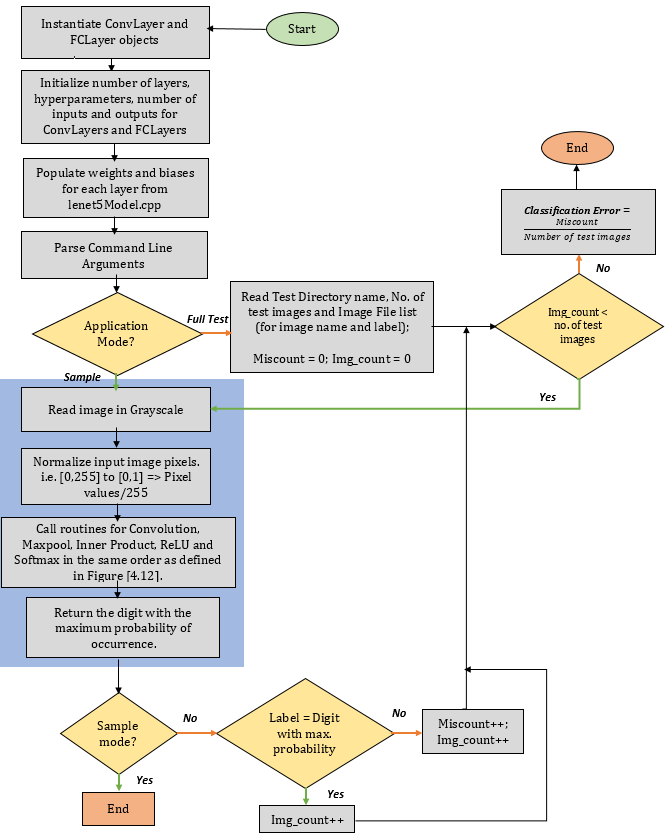
\includegraphics[width=\linewidth]{figures/CPP_flow_lenet5.png}
\caption{Software Code Flow
\cite{papaa-opencl}}
\label{fig:CPP_flow_lenet5}
\end{figure}\textbf{Compilation Steps \cite{papaa-opencl}} \newline\newline
\underline{To compile the code:}
\begin{scriptsize}
\linuxbash
\begin{lstlisting}
$ make all
\end{lstlisting}
\end{scriptsize}
\underline{To test a sample image:}
\begin{scriptsize}
\linuxbash
\begin{lstlisting}
$ ./lenet_app -m sample -i <image_path>
\end{lstlisting}
\end{scriptsize}
Example: 
\begin{scriptsize}
\linuxbash
\begin{lstlisting}
$ ./lenet_app -m sample -i ../imgs/mnist_test_img_0.pgm
\end{lstlisting}
\end{scriptsize}
\underline{To test the full MNIST Dataset:}
\begin{scriptsize}
\linuxbash
\begin{lstlisting}
$ ./lenet_app -m test -f <image_list_file> -d <image_dir> [-n <no_images_to_test>]
\end{lstlisting}
\end{scriptsize}
Example: 
\begin{scriptsize}
\linuxbash
\begin{lstlisting}
$ ./lenet_app -m test -f ../imgs/mnist_test_img_list.csv -d ../imgs/mnist-testset
\end{lstlisting}
\end{scriptsize}
The .csv image list file contains all MNIST handwritten images sized 28x28, along with their labels. These labels help calculate the prediction accuracy and error probability of the digit classifier.\newline
\textbf{Acceleration Hot-spots} \newline 
In order to identify the acceleration hot-spots, each operation of the ConvNet was profiled and the results were observed as illustrated in Table \ref{table:sw_hotspots}. The total application runtime (execution of all 8 layers) is around 77269 $\mu$s = 0.077 seconds. The API \textit{\textbf{PAPI\_get\_virt\_usec()}} is used to get the timestamp in microseconds. To use this API, header file "papi.h" has to be included in the source file.

\newcolumntype{L}[1]{>{\raggedright\arraybackslash}p{#1}}
\begin{table}[htbp]
\caption{Analysis of Application Hot-spots for Acceleration \cite{notchenko2016sparse}}
\centering
\begin{tabular}{@{}m{0.21\linewidth} m{0.21\linewidth}*{2}{L{\dimexpr0.22\linewidth-2\tabcolsep\relax}}@{}}
\toprule
& & \multicolumn{2}{c}{Execution Time (ms)} \\
\cmidrule(r{2pt}){3-4} Layers &Computational Complexity& Intel Core i3-2350M CPU @ 2.30GHz & ZedBoard CPU (2 ARM Cortex A9 Cores)\\
\midrule
Convolution 1 & 300020 &12.308&66.577\\
\midrule
MaxPool 1&2880&3.382&14.248\\
\midrule
Convolution 2 &1689000 &48.164&359.519\\
\midrule
MaxPool 2&800&0.559&4.166\\
\midrule
Inner Product 1&400500&5.522&47.924\\
\midrule
ReLU&500&0.012&0.073\\
\midrule
Inner Product 2&5010&0.073&0.609\\
\midrule
Softmax&20&0.009&0.110\\
\bottomrule
\end{tabular}
\label{table:sw_hotspots}
\end{table}

In Table \ref{table:hyperparams}, the output volume of each Layer of ConvNet is computed based on the concepts discussed in Section 3.1.1.1, given the input dimensions and hyperparameters. Each layer is studied carefully to gather the computational demand of the application. \newline \newline
For example, in the first convolution layer, filtering operation requires 288K (24 $\times$ 24 $\times$ 5 $\times$ 5 $\times$ 1 $\times$ 20) MAC operations. Feature map accumulation along the depth dimension demands another 500 (20 $\times$ 1 $\times$ 5 $\times$ 5) accumulation operations. Addition of bias to each filter output involves 11520 (20 $\times$ 1 $\times$ 24 $\times$ 24) accumulation operations. Hence, the total computational demand of the first convolution layer is estimated to be around 300K MAC operations. \newline \newline
In the MaxPool layer, the maximum value is identified in each pooling window region spanning to 2 $\times$ 2. Hence, 20 channels of 24 $\times$ 24 inputs demand a total of 20 $\times$ 12 $\times$ 12 = 2880 findMax operations in the first Maxpool layer.  The Inner Product Layer’s computational demand is dictated by the input-output dimensions. Hence, the first IP Layer involves 400K MAC operations (500 $\times$ 800) and 500 accumulations for addition of filter bias. Complexity of the ReLU and Softmax layers are dependent on the input size. \newline \newline
The convolution layer involves about 83\% of the required arithmetic operations in the ConvNet framework. Following this, the fully connected layers are the next most resource-intensive layers. \newline \newline
Table \ref{table:sw_hotspots} illustrates the computational complexity of all layers in the Lenet-5 ConvNet (Figure \ref{fig:Lenet-5-MNIST}) and their execution time in Intel Core i3-2350M CPU and Zedboard processing system containing 2 ARM Cortex A9 Cores.\newline

\begin{table}[htbp]
\caption{Inferences from Table \ref{table:sw_hotspots} for Convolution Layer 1 running on CPU}
\centering
\begin{tabular}{@{}p{0.35\linewidth}*{2}{L{\dimexpr0.3\linewidth-1\tabcolsep\relax}}@{}}
\toprule
& \multicolumn{2}{c}{Test Devices} \\
\cmidrule(r{4pt}){2-3} & \makecell[c]{Intel Core \\i3-2350M CPU} & \makecell[c]{ZedBoard ARM}\\
\midrule
Time taken for 1 MAC & \makecell[c]{$\frac{12.308 ms}{300020}$ = 41 ns} & \makecell[c]{$\frac{66.577 ms}{300020}$ = 221.9 ns} \\
\midrule
MACs/second &\makecell[c]{\\$\frac{1}{41 ns}$ = 24,390,243.9\\ \\$\approx$ 24M MACs/s} & \makecell[c]{\\$\frac{1}{221.9 ns}$ = 4,506,534.47\\ \\$\approx$ 4M MACs/s} \\
\midrule
\makecell[l]{Expected speedup with\\ hypothetical platform\\(20 processors @\\100 MHz,\\ 1MAC/cycle each)} &\makecell[c]{$\frac{12.308 ms}{150 \mu s}$ = 82.05} &\makecell[c]{$\frac{66.577 ms}{150 \mu s}$ = 443.84} \\
\bottomrule
\end{tabular}
\label{table:conv1_inference}
\end{table}

We observe from the table \ref{table:sw_hotspots} that for the first convolution layer, the execution time taken by different CPUs to compute 300,020 MAC operations gives an estimate on the number of MACs/second. Using this estimates, we assess the number of MAC operations per second as shown in Table \ref{table:conv1_inference}. 

In the software implementation, the input image is loaded from external memory. These load-stores in external memory can create a lot of data movement overheads. Hypothetically, these can be overcome by storing the images on-chip, avoiding unnecessary load-stores in external memory. 
Consider a hypothetical platform with 20 RISC processors, each capable of performing 1 MAC every cycle and running at 100 MHz.
\begin{enumerate}[label=(\roman*)]
\item Time period of 1 cycle = $\frac{1}{100 MHz}$ = 10 ns
\item Number of MACs computed by 20 RISC processors in one cycle = 20
\item Number of cycles required to compute 300020 MACs in Convolution Layer 1 by 20 RISC processors = 15001 Cycles
\item Time taken by 20 RISC processors to compute 300020 MACs in Convolution Layer 1 = 15001 $\times$ 10 ns =  150 us
\end{enumerate}

Table \ref{table:conv2_inference} illustrates inferences for convolution layer 2 from its execution time on different CPUs. Each 12 $\times$ 12 input image involves 1689 MACs (Filtering: (8 $\times$ 8 $\times$ 5 $\times$ 5) + Feature Map Accumulation: (5 $\times$ 5) + Bias Addition: (8 $\times$ 8)). 

\begin{enumerate}[label=(\roman*)]
\item Number of cycles required to compute 1689000 MACs in Convolution Layer 2 by 20 RISC processors = 84450 Cycles
\item Time taken by 20 RISC processors to compute 1689000 MACs in Convolution Layer 2 = 84450 $\times$ 10 ns =  844.5 us
\end{enumerate}

\begin{table}[htbp]
\caption{Inferences from Table \ref{table:sw_hotspots} for Convolution Layer 2 running on CPU}
\centering
\begin{tabular}{@{}p{0.35\linewidth}*{2}{L{\dimexpr0.3\linewidth-1\tabcolsep\relax}}@{}}
\toprule
& \multicolumn{2}{c}{Test Devices} \\
\cmidrule(r{4pt}){2-3} & \makecell[c]{Intel Core \\i3-2350M CPU} & \makecell[c]{ZedBoard ARM}\\
\midrule
Time taken for 1 MAC & \makecell[c]{$\frac{48.164 ms}{1689000}$ = 28.5 ns} & \makecell[c]{$\frac{359.519 ms}{1689000}$ = 212.8 ns} \\
\midrule
MACs/second &\makecell[c]{\\$\frac{1}{28.5 ns}$ = 35,087,719.3\\ \\$\approx$ 35M MACs/s} & \makecell[c]{\\$\frac{1}{212.8 ns}$ = 4,699,248.12\\ \\$\approx$ 4M MACs/s} \\
\midrule
\makecell[l]{Expected speedup with\\ hypothetical platform\\(20 processors @\\100 MHz,\\ 1MAC/cycle each)} &\makecell[c]{$\frac{48.164 ms}{844.5 \mu s}$ = 57.03} &\makecell[c]{$\frac{359.519 ms}{844.5 \mu s}$ = 425.7} \\
\bottomrule
\end{tabular}
\label{table:conv2_inference}
\end{table}
The time taken for classification of one image is 70.029 ms in Intel Core i3 platform and 493.226 ms in Zedboard. Hence, the number of images that can be classified in one second is given by:
\begin{enumerate}
\item Intel Core i3-2350M: $\frac{1}{70.029 ms} \approx$ 14 frames/second
\item Zedboard ARM Core: $\frac{1}{493.226 ms} \approx$ 2 frames/second
\end{enumerate}
In real-time applications, this speed is quite less and hence, we explore possibilities to improve the latency metric.
\subsubsection{Improvements}
\label{3_1_2_3}
One approach to minimizing data transfer to off-chip memory is by using reduced bit-width fixed point numbers, realizable by using open-source fixed point arithmetic libraries like LibFi \cite{LibFi}. This approach is very straightforward and promises speedup, reduced area and consequently reduced energy consumption. However, the specifics of this approach are beyond the scope of this thesis. \newline \newline
We intend to port the various layers of the ConvNet into fine-grained Graphics Processing Units which exhibit a high degree of data-parallelism. This requires some understanding of the OpenCL device models discussed in Section \ref{2_3_1}
Each platform comes with a ready-to-use library which may pose optimization challenges, especially when designing larger applications.  Yet another challenge is mapping, owing to differences in on-chip memory, kinds of parallelism that a particular accelerator can support and communication bandwidth. 
\subsection{Experiments with OpenCL Code}
\label{3_1_3}
\subsubsection{Pre-requisites}
\label{3_1_3_1}
\subsubsection*{OpenCL Setup in Ubuntu 14.04}
The following are required to run OpenCL Applications on the system: 
\begin{itemize}
\item Drivers to support OpenCL - Already available in current GPUs
\item OpenCL Headers
\item Vendor-specific libraries (specific to Intel, NVIDIA, AMD, etc.)
\item Installable client driver (.icd)
\item libOpenCL.so 
\end{itemize} \textbf{1. Installing OpenCL Headers \cite{opencl_headers}:} \newline
Navigate to the path \textit{/usr/include} and create a directory named CL.
\begin{scriptsize}
\linuxbash
\begin{lstlisting}
$ sudo apt-get install opencl-headers
\end{lstlisting}
\end{scriptsize}
\textbf{2. Installing vendor-specific libraries} \newline
As Intel CPU is used for our experiments, the following packages are to be installed:
\begin{itemize}
\item OpenCL™ Runtime 16.1 for Intel Core™ and Intel Xeon Processors for Ubuntu (64-bit) \cite{intel_runtime}
\item Intel SDK for OpenCL™ Applications \cite{intel_openclSDK}
\end{itemize}
After navigating to the respective installation directories, the command: 
\begin{scriptsize}
\linuxbash
\begin{lstlisting}
$ sudo ./install.sh
\end{lstlisting}
\end{scriptsize}
is used to initiate installation. \newline\newline
\textbf{Dependencies:}\newline \newline
\textbf{mono-devel} package (Installation steps summarized in \cite{mono-devel}).\newline Other missing packages are usually prompted during installation and can be installed using the command: 
\begin{scriptsize}
\linuxbash
\begin{lstlisting}
$ sudo apt-get install <package_name>
\end{lstlisting}
\end{scriptsize}
Extract the SDK tarball and navigate to the extracted directory:
\begin{scriptsize}
\linuxbash
\begin{lstlisting} 
$ tar -xzvf intel_sdk_for_opencl_2016_ubuntu_6.3.0.1904_x64.tgz
$ cd intel_sdk_for_opencl_2016_ubuntu_6.3.0.1904_x64
\end{lstlisting}
\end{scriptsize}
The rpm directory contains many default packages for RedHat Linux with \textbf{.rpm} extension. They need to be converted to \textbf{.deb}(Debian) files to be installed in Ubuntu. To handle .rpm files, \textbf{libnuma} package is required:
\begin{scriptsize}
\linuxbash
\begin{lstlisting} 
$ sudo apt-get install -y rpm alien libnuma1
\end{lstlisting}
\end{scriptsize}
To \textbf{convert rpm format to deb} format and install the Debian packages: 
\begin{scriptsize}
\linuxbash
\begin{lstlisting}        
$ alien *.rpm
$ dpkg -i *.deb 
\end{lstlisting}
\end{scriptsize}
\textbf{3. Installing the Intel OpenCL ICD Loader}
\begin{scriptsize}
\linuxbash
\begin{lstlisting}
$ sudo ln -s /opt/intel/opencl-1.2-5.2.0.10002/etc/intel64.icd /etc/OpenCL/vendors/intel64.icd
\end{lstlisting}
\end{scriptsize}
\textbf{4. Installing a symbolic link to libOpenCL.so} 
\begin{scriptsize}
\linuxbash
\begin{lstlisting}
$ sudo ln -s /opt/intel/opencl-1.2-5.2.0.10002/lib64/libOpenCL.so /usr/lib/libOpenCL.so 
$ sudo ldconfig
\end{lstlisting}
\end{scriptsize}
To check if OpenCL applications run properly, clone the GitHub repository from the link \cite{devquery} and run the Device Query program as follows:   
\begin{scriptsize}
\linuxbash
\begin{lstlisting}
$ cd OPENCL_EXAMPLES_ZEDBOARD/devquery 
$ gcc devquery.c -lOpenCL
\end{lstlisting}
\end{scriptsize}
The output should be the available devices in the system (CPU, GPU) as shown in Figure \ref{fig:DeviceQuery}.
\begin{figure}[h!]
\centering
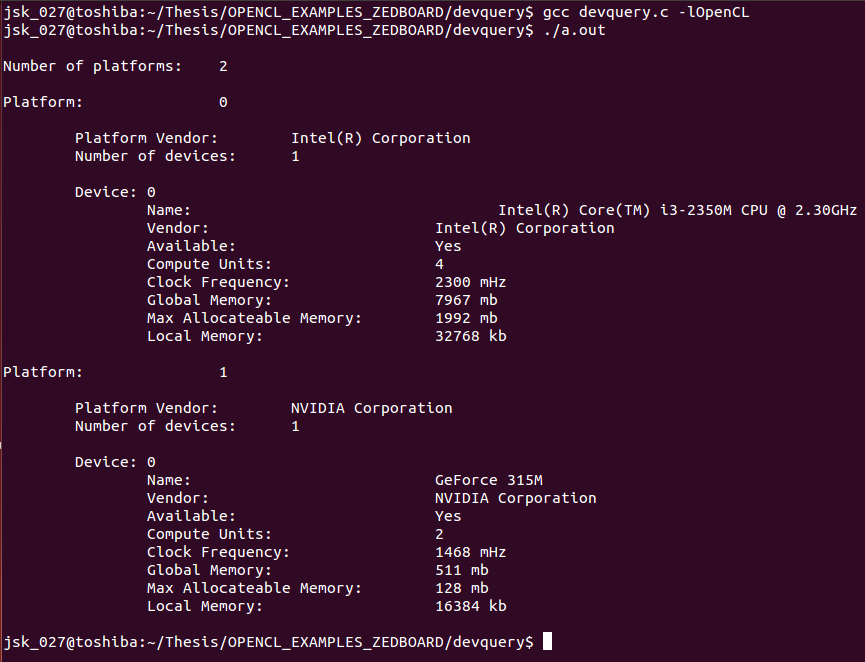
\includegraphics[width=0.7\linewidth]{figures/DeviceQuery.png}
\caption{OpenCL Device Query code Output
\cite{devquery}}
\label{fig:DeviceQuery}
\end{figure}
\subsubsection*{AOCL SDK and Quartus Installation Steps}
The FPGA Implementation of MNIST digit recognition \cite{mnist-altera-opencl} uses Altera OpenCL (AOCL) SDK (also called Intel FPGA SDK) and Quartus Software for high-level synthesis and execution. Although our experiments are not based on the Altera Platform, we may use this SDK to use some OpenCL Libraries which are independent of the hardware.\newline \newline
Intel FPGA SDK for OpenCL™ can be downloaded from \cite{opencl_fpga_sdk}. The installation steps of AOCL and Quartus from the extracted tarball are detailed in \cite{intel_fpga_guide}. Following the installation, the environment variable \textit{\$ALTERAOCLSDKROOT} is by default set to point to the path where the software was installed. A few more environment variables have to be set to inform the software of the FPGA Board in use and the runtime of the host. If the software was installed in the path, say \underline{\textit{/home/intelFPGA\_pro/17.0/hld/}}, then \textit{echo \$ALTERAOCLSDKROOT} returns the same path where software was installed. 
\begin{scriptsize}
\linuxbash
\begin{lstlisting}
$ export PATH=$ALTERAOCLSDKROOT/bin:$PATH
$ export AOCL_BOARD_PACKAGE_ROOT=/home/intelFPGA_pro/17.0/hld/board/s5_ref
$ export QUARTUS_ROOTDIR=/home/intelFPGA_pro/17.0/quartus/bin
$ export LD_LIBRARY_PATH=$ALTERAOCLSDKROOT/host/linux64/lib:$AOCL_BOARD_PACKAGE_ROOT/linux64/lib:/usr/local/lib:$LD_LIBRARY_PATH
$ source $ALTERAOCLSDKROOT/init_opencl.sh
\end{lstlisting}
\end{scriptsize}
\textit{\$AOCL\_BOARD\_PACKAGE\_ROOT} has to refer to the path of the FPGA Board in use. \textit{s5\_ref} is a reference platform available with the SDK files. When using a specific platform, the corresponding platform files are downloaded and the path of the files is used as Board Package Root. \newline \newline
The Altera.icd is copied from \textit{\$ALTERAOCLSDKROOT} to\\ \underline{\textit{/etc/OpenCL/vendors}} and the host application is linked to the ICD Loader using the following lines in the Makefile of the host.
\begin{scriptsize}
\linuxbash
\begin{lstlisting}
AOCL_LDFLAGS=$(shell aocl ldflags)
AOCL_LDLIBS=$(shell aocl ldlibs)

host_prog : host_prog.o
g++ -o host_prog host_prog.o $(AOCL_LDFLAGS) -lOpenCL $(AOCL_LDLIBS)
\end{lstlisting}
\end{scriptsize}

\subsubsection{Existing Code Flow Description}
\label{3_1_3_2}
\begin{figure}[h!]
\centering
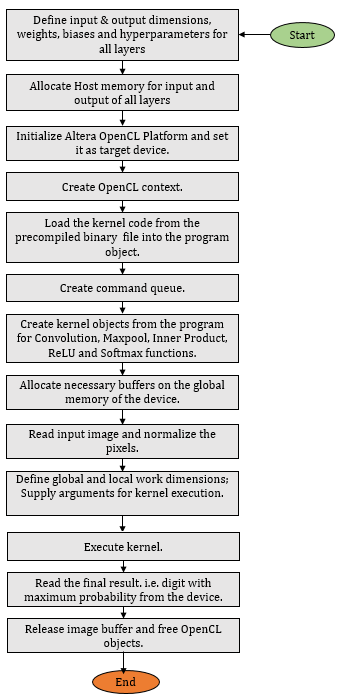
\includegraphics[width=0.5\linewidth]{figures/opencl_flow_lenet5.png}
\caption{OpenCL code flow for Sample (single image recognition) mode \cite{mnist-altera-opencl}}
\label{fig:opencl_flow_lenet5}
\end{figure}
The OpenCL implementation of MNIST/Lenet-5 architecture available in the repository \cite{mnist-altera-opencl} is specific to Altera FPGA devices. In order to make this implementation generic and executable on CPU and GPU, the existing code flow has been examined. Figure \ref{fig:opencl_flow_lenet5} shows the sequence of steps that are done when the a sample image has to be identified.\newline \newline
The first step is the initialization of parameters for all layers in the CNN. This is followed by allocation of buffers necessary for storing inputs and outputs of all layers on the global memory of the device, which is also accessible by the host. The function \textit{ findPlatform()} searches for relevant strings such as Intel FPGA SDK for OpenCL, Altera SDK, etc. When a match-word "Altera" is given as argument to this function, it looks for an Altera platform. Should the platform be available, the next step is to query all OpenCL devices in this platform and set one of them as the target device. \newline\newline
The OpenCL Runtime Environment requires a \textbf{context} to manage memory, program, command issue, kernels, and program execution on the device for which the context is defined. Following the context creation, the source code to be ported to GPU is read into a program object.\newline\newline
There are two ways to compile a kernel \cite{opencl_book_html}. \textbf{Online compilation} involves reading of the kernel source code by the host and building of the source code at runtime, by the OpenCL Runtime library. For this, the API \textit{clCreateProgramWithSource()} is used, followed by the API \textit{clBuildProgram()}. This method is not recommended for real-time embedded applications. If the kernel is pre-compiled using an OpenCL compiler, the kernel binary is already available and is directly read by the host program, skipping the runtime compilation. This is called \textbf{Offline compilation} and requires only one OpenCL function \textit{clCreateProgramWithBinary()}. Although this saves the time to compile the kernel source during runtime, it is platform-specific. If the same kernel code is to be offloaded to other platforms, then a different set of binaries should be generated. Inclusion of multiple kernel binaries increases the size of the executable.
\begin{figure}[h!]
\centering
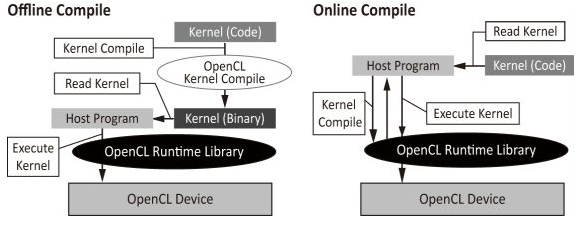
\includegraphics[width=0.7\linewidth]{figures/kernel_compilation.PNG}
\caption{Kernel Compilation Modes \cite{opencl_book_html}}
\label{fig:kernel_compilation}
\end{figure}
The reference code \cite{mnist-altera-opencl} is specific to Altera devices and uses an offline compilation flow, due to the availability of pre-compiled binary.\newline\newline
Next, a \textbf{command queue} is created which instructs which command has to be executed in which device of the group of devices in a particular context. It also dictates whether the execution should occur in-order or out-of-order. Because the intention is to accelerate the entire ConvNet, kernel objects are created for Convolution, Maxpooling, Inner Product and Activation Layers (ReLU and Softmax). Enough memory has to allocated on the OpenCL device to support the weights, biases, I/Os and execution of kernel calls for all 8 layers of the Lenet-5 Model. \newline\newline
The input image pixels are read and normalized. The kernel code is executed on the device and the final result, i.e. the digit with maximum likelihood is read from the device. Finally, the buffers and memory objects freed.
\subsubsection{Modifications to remove Platform Dependencies}
\label{3_1_3_3}
\textbf{Allocation of Buffers on the Device Memory:}\newline
For Altera FPGAs, the Altera Offline Compiler (AOC) is responsible for generation of logic to support memory accesses \cite{alteraopencl}. 
\begin{figure}[h!]
 \centering
 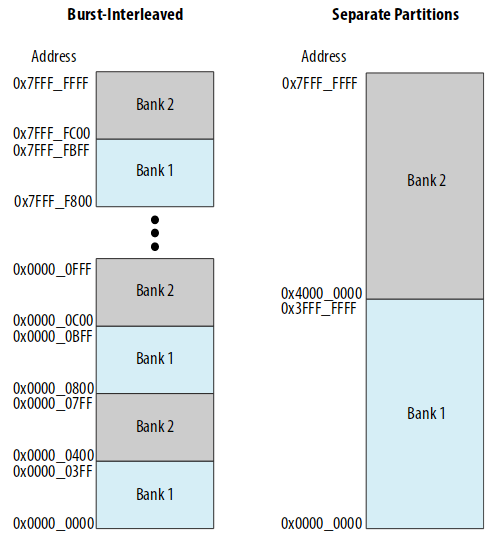
\includegraphics[width=0.5\linewidth]{figures/global_mem_partitions.png}
 \caption{Default (bus-interleaved) vs. Manual Global Memory Partitioning
 \cite{alteraopencl}}
 \label{fig:global_mem_partitions}
\end{figure}
It uses the device SDRAM as global memory and by default, stores the data in a burst-interleaved fashion across various external memory banks. Although this offers uniform load distribution and better balance between the banks, manual partitioning of the data may come in handy for certain applications. For example, when the memory banks support different data-types, data cannot be impartially interleaved to these banks. \newline \newline
The MNIST-Altera code \cite{mnist-altera-opencl} accesses global memory using optimized memory banks instead of default burst data allocation in the global memory. 
For efficient global memory access, the weights and biases are stored in Bank 2 while the data is stored in Bank 1. However, the memory banks in the GPU context refer to partitioning of shared memory into equal blocks which can be accessed simultaneously. Bank conflicts due to certain access patterns can slow down the GPU performance \cite{gpu_mem_bank}. Hence, the first step to removing platform dependencies is removal of flags CL\_MEM\_BANK\_1\_ALTERA and CL\_MEM\_BANK\_2\_ALTERA which characterize Altera memory banks (Refer \ref{cnncode1:altera-dep-removal}).\newline \newline
\definecolor{hg}{rgb}{0.75,1.0,0.75}
\definecolor{hr}{rgb}{1.0,0.92,0.8}
\newcommand{\grn}{\makebox[0pt][l]{\color{hg}\rule[-4pt]{0.9\linewidth}{10pt}}}
\newcommand{\rd}{\makebox[0pt][l]{\color{hr}\rule[-4pt]{0.9\linewidth}{10pt}}}
\lstset { %
	language=C,
	backgroundcolor=\color{white},
	basicstyle=\ttfamily\tiny,
	keywordstyle=\color{magenta}\ttfamily,
	stringstyle=\color{blue}\ttfamily,
	commentstyle=\color{green}\ttfamily,
    breakatwhitespace=false,
	breaklines=true,
    showstringspaces=false, 
    escapeinside={<@}{@>}
}
\noindent\begin{minipage}{.45\textwidth}
\begin{lstlisting}[caption=Header files for Altera FPGA,frame=tlrb]{Name}
#include <stdio.h>
#include <stdlib.h>
#include <iostream>
#include <iomanip>
#include <fstream>
#include <unistd.h>
#include <math.h>
<@\textcolor{red}{\textbf{\#include "CL/opencl.h"}}@>
<@\textcolor{red}{\textbf{\#include "AOCLUtils/aocl\_utils.h}}@>
#include "cnn_structs.h"
#include "pgm.h"
#include "lenet5_model.h"

<@\textcolor{red}{\textbf{using namespace aocl\_utils;}}@>
using namespace std;
\end{lstlisting}
\end{minipage}\hfill
\begin{minipage}{.45\textwidth}
\begin{lstlisting}[caption=Header files for \\ GPU,frame=tlrb]{Name}
#include <stdio.h>
#include <stdlib.h>
#include <iostream>
#include <iomanip>
#include <fstream>
#include <unistd.h>
#include <math.h>
<@\textcolor{green}{\textbf{\#include <CL/cl.h>}}@>
<@\textcolor{green}{\textbf{\#include <CL/cl\_ext.h>}}@>
#include "cnn_structs.h"
#include "pgm.h"
#include "lenet5_model.h"

using namespace std;
\end{lstlisting}
\end{minipage}\newline
\textbf{Usage of Generic OpenCL headers} \newline
Although AOCL Utility is a platform independent C++ header file, it has been replaced with standard OpenCL headers for the sake of generality. All APIs in the scope of AOCL Utility namespace are substituted by general OpenCL APIs described in \cite{opencl_khronos}. \newline \newline
\textbf{Kernel Loading Mechanism}\newline
On-the-fly kernel loading, i.e. Online compilation method explained in subsection \ref{3_1_3_2} is employed. The existing and modified code changes are depicted clearly in \ref{cnncode2:load-kernel-source}, \ref{cnncode3:altera-opencl-init} and \ref{cnncode4:gpu-opencl-init}.\newline \newline
\textbf{Changes to Makefile}\newline
Altera platform specific libraries are unlinked. \textit{libOpenCL.so} Shared Library is linked in the Makefile as shown in Figure \ref{fig:makefile}. The resultant code is free from any dependencies with Altera platform and hence, can be compiled and run on any OpenCL device.
\begin{figure}[h!]
\centering
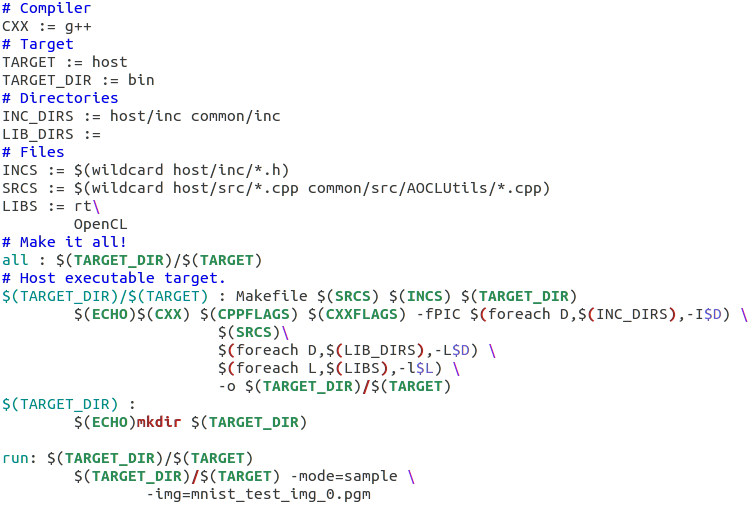
\includegraphics[width=0.7\linewidth]{figures/makefile.png}
\caption{Linking libOpenCL Library to Makefile}
\label{fig:makefile}
\end{figure}
\subsubsection{Compiling and executing the code}
\label{3_1_3_4}
\underline{To test a sample image:}\newline
\begin{scriptsize}
\linuxbash
\begin{lstlisting}
$ make run
\end{lstlisting}
\end{scriptsize}
\underline{To test the full MNIST Dataset:}\newline
\begin{scriptsize}
\linuxbash
\begin{lstlisting}
$ make test
\end{lstlisting}
\end{scriptsize}
The path of the test images (sample and full dataset) is also supplied to the host through the Makefile. Hence, the path has to be suitably modified to point to the test images in the local machine.\newline\newline
The kernels can be executed either in CPU or GPU devices which support OpenCL.\newline
\hfill
\begin{minipage}{\textwidth}
\begin{center}
\begin{lstlisting}[caption= CPU or GPU Device Selection,frame=tlrb, basicstyle = \small]{Name}
int gpu = 1;
for(unsigned i = 0;i < dev_cnt; i++){
   err = clGetDeviceIDs(platform_ids[i], gpu ? CL_DEVICE_TYPE_GPU : CL_DEVICE_TYPE_CPU, 1, &target_device, NULL);
   if(err == CL_SUCCESS){
      break;
   }
}
\end{lstlisting}
\end{center}
\end{minipage}
When the integer variable \textit{'gpu'} is set to 1, the GPU device is selected and when it is set to 0, the CPU device is selected.
\subsubsection*{Benchmarking Kernel Execution Time}
\begin{itemize}
\item Profiling should be enabled during the creation of command queue as follows:\\
\begin{minipage}{\textwidth}
\begin{center}
\begin{lstlisting}[columns=fullflexible, language=C++, escapechar = \$, backgroundcolor=\color{gray!10}, basicstyle = \small]
queue = clCreateCommandQueue(context, target_device, $\textcolor{red}{CL\_QUEUE\_PROFILING\_ENABLE}$, &status); 
checkError(status, "Failed to create command queue");
\end{lstlisting}
\end{center}
\end{minipage}
\item An event is associated with the kernel during its launch as follows:\\
\begin{minipage}{\textwidth}
\begin{center}
\begin{lstlisting}[columns=fullflexible, language=C++, escapechar = \$, backgroundcolor=\color{gray!10}, basicstyle = \small]
status = clEnqueueNDRangeKernel(queue, kernel[0], 3, NULL, global_work_size, NULL, 0, NULL, $\textcolor{red}{\&kernel\_event[0]}$);
checkError(status, "Failed to launch conv1 kernel");
\end{lstlisting}
\end{center}
\end{minipage}
\item Kernel execution has to be completed and also all enqueued tasks in the command queue should finish.\\
\begin{minipage}{\textwidth}
\begin{center}
\begin{lstlisting}[columns=fullflexible, language=C++, escapechar = \$, backgroundcolor=\color{gray!10}, basicstyle = \small]
clWaitForEvent(1, &kernel_event[0]);
clFinish(queue);
\end{lstlisting}
\end{center}
\end{minipage}
\item The following APIs can be used to estimate the kernel execution time:\\
\begin{minipage}{\textwidth}
\begin{center}
\begin{lstlisting}[columns=fullflexible, language=C++, escapechar = \$, backgroundcolor=\color{gray!10}, basicstyle = \small]
cl_ulong start_time, end_time;
double total_time;
clGetEventProfilingInfo(kernel_event[0], CL_PROFILING_COMMAND_START, sizeof(start_time), &start_time, NULL);
clGetEventProfilingInfo(kernel_event[0], CL_PROFILING_COMMAND_END, sizeof(end_time), &end_time, NULL);
total_time = end_time-start_time;
printf("Kernel Execution Time is: %0.3f \n",total_time/1000000.0);
\end{lstlisting}
\end{center}
\end{minipage}
\end{itemize}
\subsection{Comparative Study of Results}
A simple device query program is run on each of the test devices to query attributes such as memory, number of compute units, etc. The test device specifications are tabulated for comparison in Table \ref{table:dev_query}. 
\label{3_1_4}
\newcolumntype{L}[1]{>{\raggedright\arraybackslash}p{#1}}
\begin{table}[htbp]
\caption{Test Device Specifications}
\centering
\begin{tabular}{@{}p{0.25\linewidth}*{4}{L{\dimexpr0.15\linewidth-1\tabcolsep\relax}}@{}}
\toprule
& \multicolumn{4}{c}{Test Devices} \\
\cmidrule(r{4pt}){2-5}Attributes & Intel Core i3-2350M CPU & NVIDIA GeForce 315M & Intel Xeon CPU E5-1650 & NVIDIA Quadro 600\\
\midrule
OpenCL Version & \makecell[c]{1.2} & \makecell[c]{1.1} & \makecell[c]{2.1} & \makecell[c]{1.1}\\
\midrule
Compute Units &\makecell[c]{4} &\makecell[c]{2} & \makecell[c]{12} & \makecell[c]{2}\\
\midrule
\makecell[l]{Clock\\Frequency (MHz)} &\makecell[c]{2300} &\makecell[c]{1468} & \makecell[c]{3200} & \makecell[c]{1280}\\
\midrule
\makecell[l]{Global Memory\\(MB)} &\makecell[c]{7967} &\makecell[c]{511} & \makecell[c]{15971} & \makecell[c]{1023}\\
\midrule
\makecell[l]{Maximum\\Allocateable\\ Memory (MB)}&\makecell[c]{1992} &\makecell[c]{128} & \makecell[c]{3993} & \makecell[c]{256}\\
\midrule
\makecell[l]{Local Memory\\(KB)} &\makecell[c]{32768} &\makecell[c]{16384} & \makecell[c]{32768} & \makecell[c]{49152}\\
\bottomrule
\end{tabular}
\label{table:dev_query}
\end{table}

\begin{table}[htbp]
\caption{Comparison of kernel runtime in various OpenCL Devices}
\centering
\begin{tabular}{@{}p{0.21\linewidth}*{4}{L{\dimexpr0.15\linewidth-1\tabcolsep\relax}}@{}}
\toprule
& \multicolumn{4}{c}{Kernel Execution Time (ms)} \\
\cmidrule(r{4pt}){2-5} & Intel Core i3-2350M CPU & NVIDIA GeForce 315M & Intel Xeon CPU E5-1650 & NVIDIA Quadro 600\\
\midrule
Convolution 1 & \makecell[c]{0.216} & \makecell[c]{0.707} & \makecell[c]{0.088} & \makecell[c]{0.143}\\
\midrule
MaxPool 1 &\makecell[c]{0.046} &\makecell[c]{0.166} & \makecell[c]{0.022} & \makecell[c]{0.029}\\
\midrule
Convolution 2 &\makecell[c]{0.716} &\makecell[c]{11.332} & \makecell[c]{0.146} & \makecell[c]{1.846}\\
\midrule
Maxpool 2 &\makecell[c]{0.026} &\makecell[c]{0.371} & \makecell[c]{0.014} & \makecell[c]{0.026}\\
\midrule
Inner Product 1&\makecell[c]{0.187} &\makecell[c]{1.651} & \makecell[c]{0.039} & \makecell[c]{1.747}\\
\midrule
ReLU &\makecell[c]{0.011} &\makecell[c]{0.012} & \makecell[c]{0.007} & \makecell[c]{0.005}\\
\midrule
Inner Product 2&\makecell[c]{0.010} &\makecell[c]{0.287} & \makecell[c]{0.006} & \makecell[c]{0.109}\\
\midrule
Softmax &\makecell[c]{0.014} &\makecell[c]{0.012} & \makecell[c]{0.008}& \makecell[c]{0.007}\\
\bottomrule
\end{tabular}
\label{table:results_compare_cnn}
\end{table}

\textbf{Goal:} Achieve a faster runtime in hardware compared to software.
The ratio $R_{acceleration}$ = $\frac{t_{sw}}{t_{hw}} \textgreater $ 1\newline 
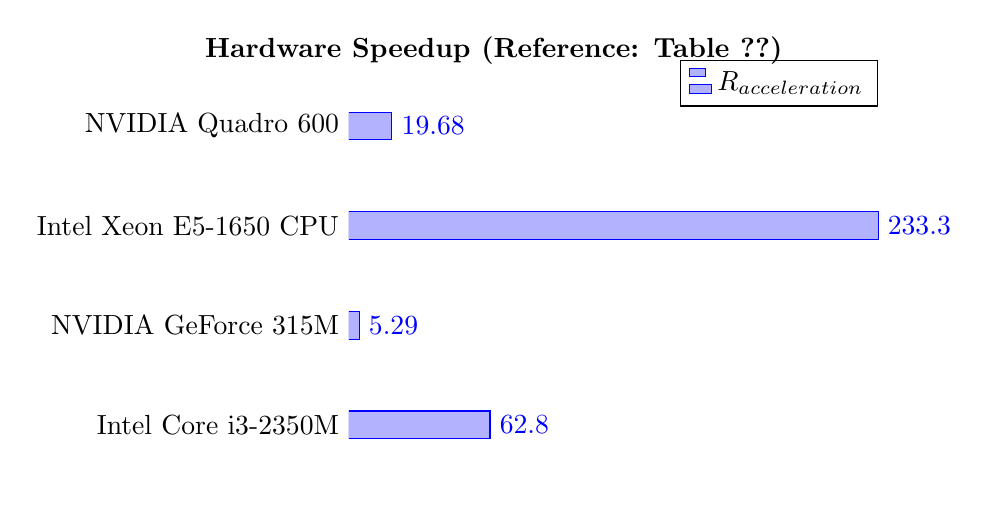
\begin{tikzpicture}
  \begin{axis}[xbar,
    y axis line style = { opacity = 0 },
    axis x line       = none,
    tickwidth         = 0pt,
    enlarge y limits  = 0.25,
    enlarge x limits  = 0.02,
    symbolic y coords = {Intel Core i3-2350M, NVIDIA GeForce 315M, Intel Xeon E5-1650 CPU, NVIDIA Quadro 600},
    nodes near coords,
  ]
  \addplot coordinates { 
  (62.8,Intel Core i3-2350M)         
  (5.29,NVIDIA GeForce 315M)                       
  (233.3,Intel Xeon E5-1650 CPU)
  (19.683,NVIDIA Quadro 600)
  };
  \legend{$R_{acceleration}$}
  \end{axis}
  % title
\node[align=center,font=\bfseries](title) at (current bounding box.north)
{Hardware Speedup (Reference: Table \ref{table:results_compare_cnn})};
\end{tikzpicture}
\newline The total time required to classify one input image is 1.21ms in Intel Core i3-2350M, 14.526ms in NVIDIA GeForce 315M, 3.905ms in NVIDIA Quadro 600 and 322 us in Intel Xeon platform. This implies that in one second, the number of images that can be processed by each of these heterogeneous platforms is given by:
\begin{enumerate}
\item Intel Core i3-2350M:  $\frac{1}{1.21ms} \approx$ 826 frames/second
\item NVIDIA GeForce 315M:  $\frac{1}{14.526ms} \approx$ 68 frames/second
\item Intel Xeon CPU E5-1650: $\frac{1}{0.322ms} \approx$ 3105 frames/second
\item NVIDIA Quadro 600: $\frac{1}{3.905ms} \approx$ 256 frames/second
\end{enumerate}

\begin{table}[htbp]
\caption{Inferences from execution times of OpenCL devices running offloaded Convolution Layer 1 code (Calculations similar to Tables \ref{table:conv1_inference} and \ref{table:conv2_inference})}
\centering
\begin{tabular}{@{}p{0.4\linewidth}*{4}{L{\dimexpr0.15\linewidth-1\tabcolsep\relax}}@{}}
\toprule
& \multicolumn{4}{c}{Test Devices} \\
\cmidrule(r{4pt}){2-5} & \makecell[c]{Intel\\Core\\i3-2350M} & \makecell[c]{NVIDIA\\GeForce\\315M} & \makecell[c]{Intel\\Xeon\\CPU\\E5-1650}&\makecell[c]{NVIDIA\\Quadro\\600}\\
\midrule
Time taken for 1 MAC & \makecell[c]{0.7 ns} & \makecell[c]{2.35 ns} &\makecell[c]{0.29 ns} & \makecell[c]{0.47 ns}\\
\midrule
MACs/second (approx.) &\makecell[c]{1 B} & \makecell[c]{400 M} &\makecell[c]{3 B} &\makecell[c]{2 B}\\
\midrule
\makecell[l]{Gained Speedup compared\\to Intel Core i-3 running\\ single-threaded C++ code} &\makecell[c]{56.98} &\makecell[c]{17.4}&\makecell[c]{139.86} &\makecell[c]{86.069} \\
\midrule
\makecell[l]{Gained Speedup compared\\to Zedboard ARM running\\single-threaded C++ code} &\makecell[c]{308.2} &\makecell[c]{94}&\makecell[c]{756.5} &\makecell[c]{465.57} \\
\midrule
\makecell[l]{Expected speedup with\\ hypothetical platform\\(20 processors @ 100 MHz,\\1 MAC/cycle each)} &\makecell[c]{1.44} &\makecell[c]{4.7}&\makecell[c]{0.58} &\makecell[c]{0.95} \\
\bottomrule
\end{tabular}
\label{table:opencl_conv1_inference}
\end{table}

In summary, it can be observed from Table \ref{table:conv1_inference} that when running single-threaded C++ code for convolution layer 1, the hypothetical platform is approximately 82 times faster than Intel core-i3 and 440 times faster than Zedboard ARM. Table \ref{table:conv2_inference} estimates reveal that the time required for the hypothetical platform to get all outputs of Convolution Layer 2 is 57 times faster than Intel core-i3 platform and 426 times faster than Zedboard ARM for convolution layer 2. \newline \newline
A close observation of Tables \ref{table:dev_query} and \ref{table:results_compare_cnn} shows that with more memory to work on and more compute units, more threads can be concurrently executed and hence, more speedup can be achieved. \newline \newline
When the same CNN code is offloaded to an OpenCL device capable of executing multiple threads in parallel, the gain in latency is enormous, almost comparable to our hypothetical platform. For example, the same convolution algorithm running on the same platform, Intel Core i-3 CPU offers different latencies depending on whether it is a sequential execution or multi-threaded concurrent execution on several compute units. The OpenCL code is approximately 57 times faster than its single-threaded C++ counterpart (Reference: Table \ref{table:opencl_conv1_inference}). Executing work items on several low-power compute units not only improves latency but also allows CPU to perform other critical tasks. These heterogeneous architectures allow complex applications to be made more practical and hence drive today's technology roadmap.